\subsection{Following one composition through the predictor}
Consider $\mathrm{InTiO_3}$, the first-ranked seed-26 mixture candidate in the Q3 validation subset. Its actual zero gap is available only when we evaluate the prediction. During screening, the classifier puts probability 0.5426 on a positive gap. The two regressors then disagree by 9.3786 score units. Figure~\ref{fig:gate} traces the two weighted contributions in Eq.~\eqref{eq:mix} and compares their sum with the public DFT-derived loss.

\begin{figure}[htbp]
\centering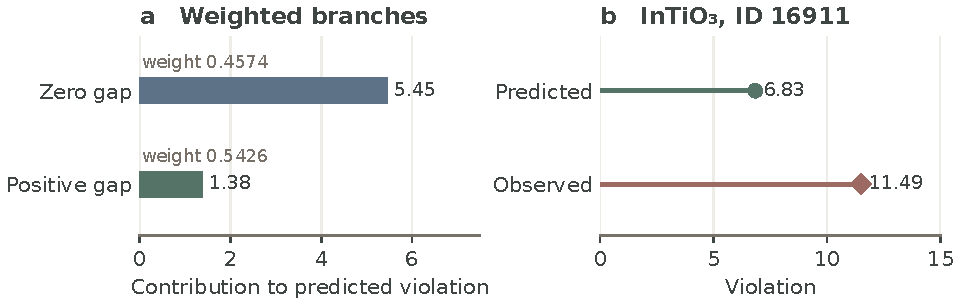
\includegraphics[width=\linewidth]{figures/gate_mechanism.pdf}
\caption{The composition-only gate for validation ID 16911 assigns positive-gap probability 0.5426. The bars give the contributions after weighting. The public loss was used only for evaluation.}\label{fig:gate}
\end{figure}

Writing $m$ and $u$ for the clipped metallic and positive-gap scores, respectively, gives $\Vh=m-p(m-u)$. The metallic branch contributes approximately $0.4574(11.9231)=5.45$ and the positive-gap branch $0.5426(2.5444)=1.38$. The arithmetic explains two features of this selection. First, a hard decision at $p=0.5$ would report only 2.5444, discarding a material portion of the expected violation. Second, a 0.10 increase in the positive-gap probability would lower the score by 0.938 with both branch estimates fixed. That sensitivity is large enough to matter among closely ranked candidates.

The gate also imposes a one-sided condition on very low scores. Since $u\geq0$ and $m\geq L$, Eq.~\eqref{eq:mix} gives
\[
 \Vh\geq (1-p)L,\qquad
 \Vh<1\ \Longrightarrow\ p>1-1/L\simeq0.9080 .
\]
This is a necessary condition on a \emph{predicted} score below one. A physically good but uncertain material may still receive a much larger score. Ranking by the continuous mixture keeps that material available when no candidate crosses a fixed prediction threshold. Conversely, assigning probability greater than 0.908 does not guarantee good band alignment or formation energy.

\subsection{A controlled test of the probability gate}
To isolate the effect of gating, we hold the learned branch functions $u$ and $m$, the seed, descriptors and train--validation split fixed. Only the mixing weight changes across the comparisons in Table~\ref{tab:gate}. The constant rule assigns the file-02 positive-gap fraction $432/11256$ to every composition. The hard rule replaces the predicted probability by $\mathbf{1}[p\geq0.5]$. The soft rule uses $p$ itself. A fourth, diagnostic rule routes each validation record by its observed gap label, an input unavailable on the blind pool. Replaying the soft rule reproduces all 3,969 archived validation scores within $10^{-8}$.

\begin{table}[htbp]
\caption{Changing only the gate on file 03. Hits count $V<1$ among the first 50. All-family and Q3 denominators are 27 and 11 available near-targets. The final column gives observed $V$ at Q3 rank one.}\label{tab:gate}
\centering\small\begin{tabular}{lrrrr}
\toprule Routing weight & All-family MAE & All hits & Q3 hits & Q3 first $V$\\\midrule
Training prevalence & 2.942 & 4 & 2 & 10.895\\
Hard decision & 2.909 & 8 & 1 & 11.492\\
Soft probability & 2.949 & 13 & 5 & 11.492\\
Observed gap (diagnostic) & 2.678 & 20 & 9 & 1.488\\\bottomrule
\end{tabular}
\end{table}

The hard decision gives a slightly smaller mean error than the soft mixture, yet it retrieves five fewer near-targets at budget 50 across all families. Many promising compositions fall below the hard threshold. Of the 141 validation materials with a positive gap, the classifier flags only 14 at $p\geq0.5$, alongside four false positives. Its precision there is $14/18$, while its recall is $14/141$. A hard rule makes the 127 missed positive-gap records share the metallic scoring regime with most of the validation set.

As a probability score for the positive-gap event, the gate attains a Brier score of 0.0273, compared with 0.0343 for the constant training prevalence. Average precision is 0.367 against a validation event frequency of 0.0355. These metrics assess the positive-gap event. No exact contest target occurs in the public labels. On Q3, even access to the observed regime yields a first choice with $V=1.4884$, above the near-target threshold. Improving the gate alone would still leave the regression problem of ranking positive-gap materials by their joint physical penalties.
